%%%%Internal Cryogenics%%%%
\label{sec:fdsp-tc-internal-cryo}

The internal cryogenics comprises three sets of pipe distribution networks and two sets of sprayers. All pipes enter the cryostat from the top; some go all the way down to the floor, and others remain in the ceiling. On the floor are:
\begin{itemize}
\setlength\itemsep{1mm}
\setlength{\parsep}{1mm}
\setlength{\itemsep}{-5mm}
\item \textbf{\dword{gar} distribution}: a set of pipes %flowing 
for \dword{gar}. These pipes are used only prior to filling %at the beginning 
to remove air %that fills 
in the cryostat. They will all have either a longitudinal slit or calibrated holes to distribute \dword{gar} uniformly along the length of the cryostat. 
\dword{cfd} simulations show that air will be removed from the system as long as \dword{gar} is flowing in at the right speed, calculated and experimentally verified as \SI{1.2}{m/hr} (vertical meters in the cryostat).  


\item \textbf{\dword{lar} distribution}: two sets of pipes are required for flowing 
\dword{lar} over a broad  range of flow rates. These pipes are used to fill the cryostat and, during steady state operations, to return the \dword{lar} from the purification system. The pipes have calibrated holes to return the \dword{lar} uniformly throughout the length of the cryostat. This is very important %for 
to maintain uniform purity. Four pumps circulate the \dword{lar} inside the cryostat, all of which operate %. Initially, all of pumps operate at once 
initially to achieve purity; %but 
once the target purity is achieved, only one or two pumps remain in service. %Two sets of pipes are needed to adequately distribute the \dword{lar} over this broad range of flow rates.
\end{itemize}

On the ceiling are:

\begin{itemize}
\setlength\itemsep{1mm}
\setlength{\parsep}{1mm}
\setlength{\itemsep}{-5mm}
\item \textbf{Cool down sprayers}: Two sets of cool down sprayers are distributed along the long sides of each cryostat. One set distributes \dword{lar} using liquid sprayers that generate a conical profile of small droplets of liquid. The other set of sprayers distributes \dword{gar} to move the \dword{lar} droplets inside and cool down the detector and cryostat uniformly. These sprayers are being tested in \dword{pddp}. They are a variation of those implemented in \dword{pdsp}.
\end{itemize}

Figure~\ref{fig:internal-cryo-3D} shows the current layout of the internal cryogenics. 
%The current drawing of the internal cryogenics is presented in Figure~\ref{fig:internal-cryo-drawing}. 
The \dword{gar} pipes are in red, the \dword{lar} pipes in blue.

\begin{dunefigure}[Layout of the internal cryogenics piping]{fig:internal-cryo-3D}
  {Layout of the internal cryogenics piping.}
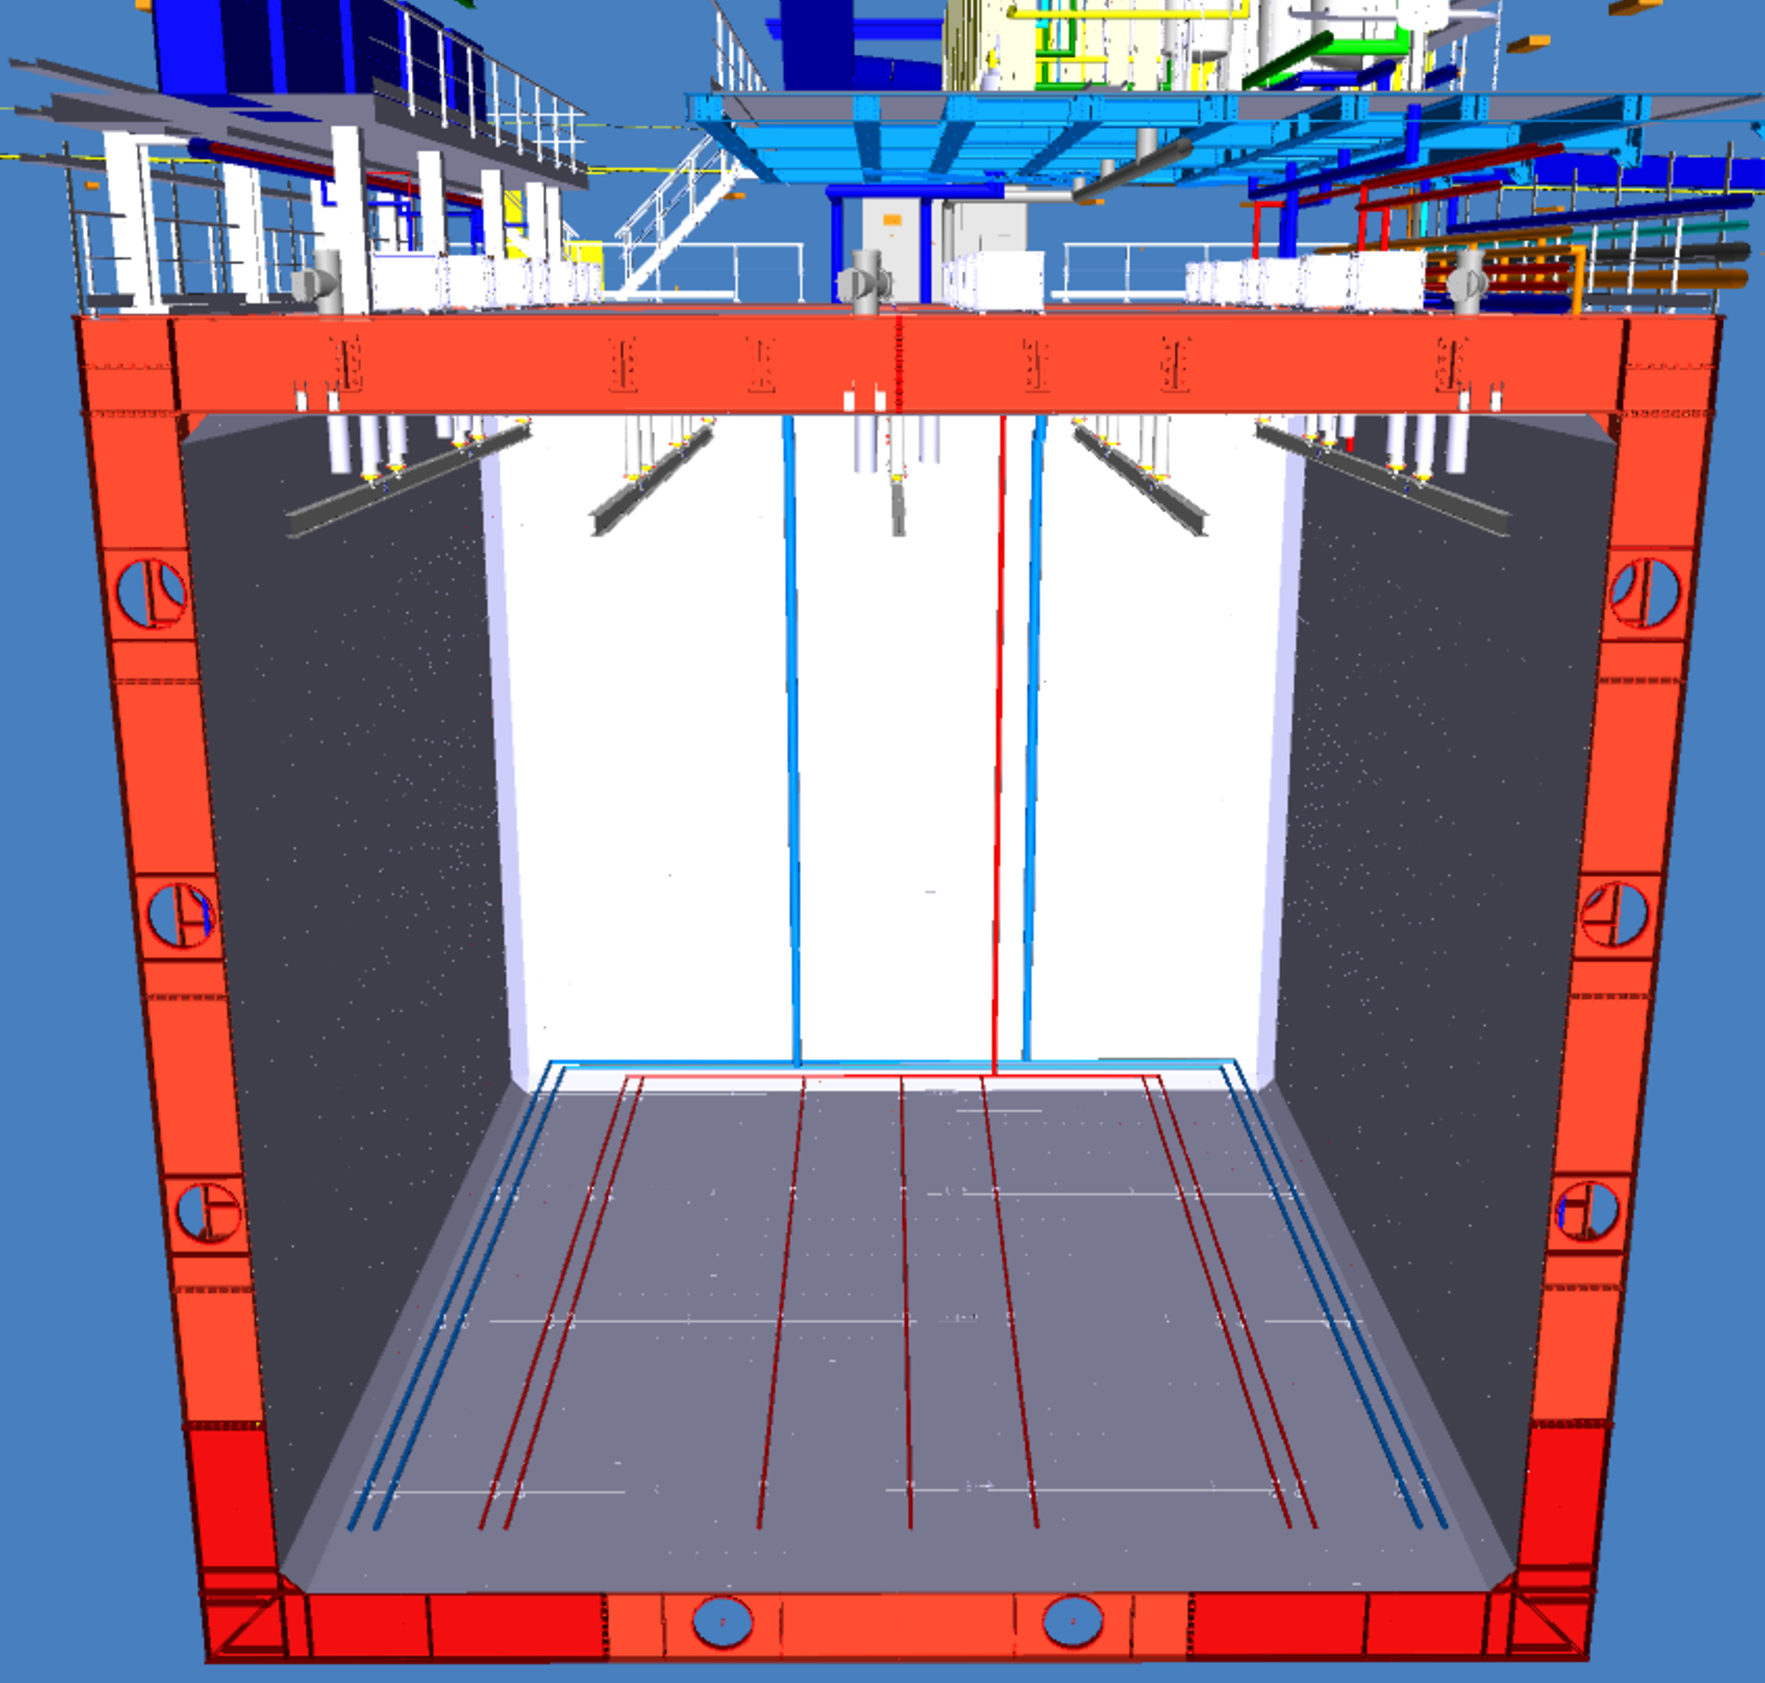
\includegraphics[width=.98\textwidth]{graphics/Internal-Piping-3D.pdf}
\end{dunefigure}

%\begin{dunefigure}[Drawing of the cryogenic %piping inside the cryostat %]{fig:internal-cryo-drawing}
%  {Drawing of the internal cryogenics.}
%\includegraphics[angle=90,width=.98\textwidth]{%graphics/Internal-pipes-HQ.pdf}
%\includegraphics[angle=90,height=.98\textheight%]{graphics/Internal-pipes-HQ.pdf}
%\end{dunefigure}
%\fixme{Please reduce size of Internal-pipes-HQ.pdf}
